\begin{figure}[t]
	\centering
	\begin{subfigure}{0.31\textwidth}
		\centering
		\includegraphics[width=\textwidth]{figures/S1-true-W.pdf}
		\caption{True Adjacency Matrix}
	\end{subfigure}
	\begin{subfigure}{0.31\textwidth}
		\centering
		\includegraphics[width=\textwidth]{figures/S3-posterior-W.pdf}
		% \caption{S3 ($T$: 18, $F$: 0.7717)}
		\caption{S3 ($T$: 18)}
	\end{subfigure}
	\begin{subfigure}{0.31\textwidth}
		\centering
		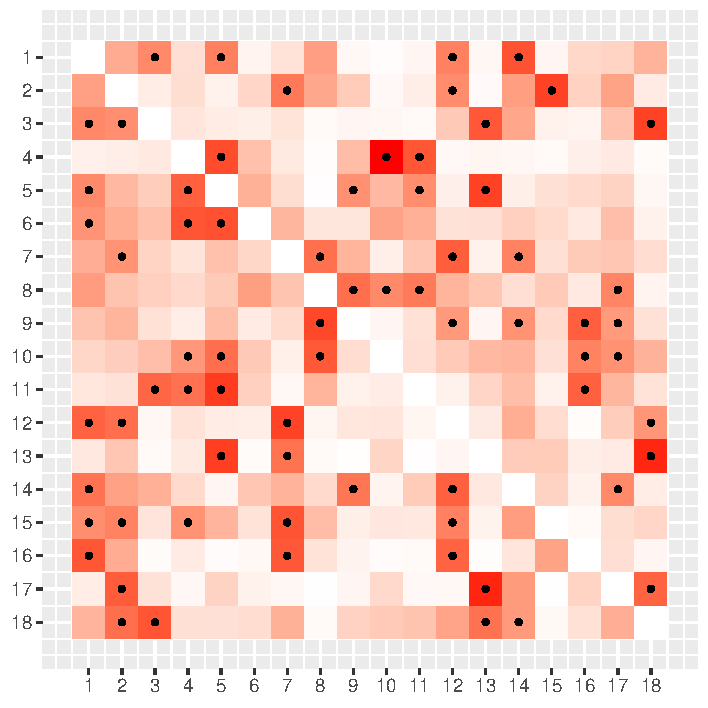
\includegraphics[width=\textwidth]{figures/S12-posterior-W.pdf}
		% \caption{S12 ($T$: 16, $F$: 0.7419)}
		\caption{S12 ($T$: 16)}
	\end{subfigure}
	\begin{subfigure}{0.31\textwidth}
		\centering
		\includegraphics[width=\textwidth]{figures/S9-posterior-W.pdf}
		% \caption{S9 ($T$: 12, $F$: 0.5848)}
		\caption{S9 ($T$: 12)}
	\end{subfigure}
	\begin{subfigure}{0.31\textwidth}
		\centering
		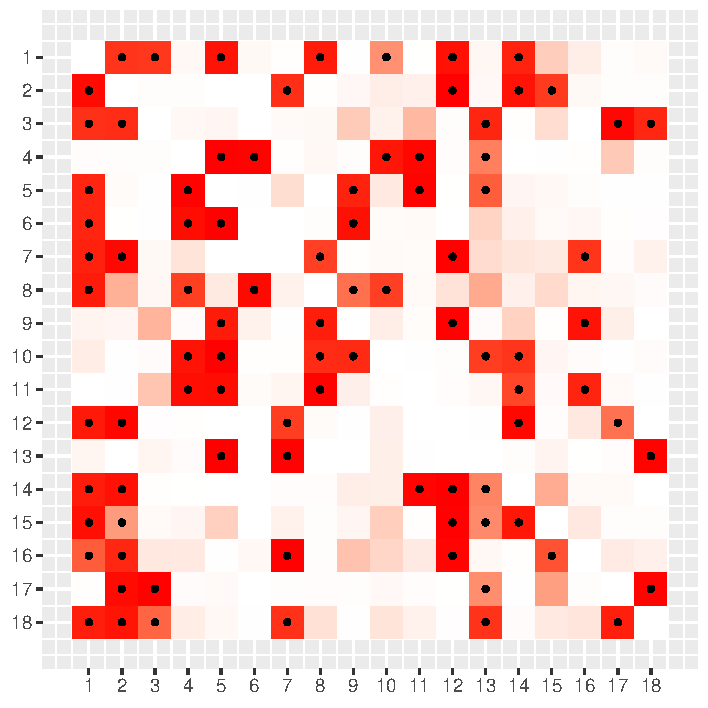
\includegraphics[width=\textwidth]{figures/S10-posterior-W.pdf}
		% \caption{S10 ($T$: 8, $F$: 0.5258)}
		\caption{S10 ($T$: 8)}
	\end{subfigure}
	\begin{subfigure}{0.31\textwidth}
		\centering
		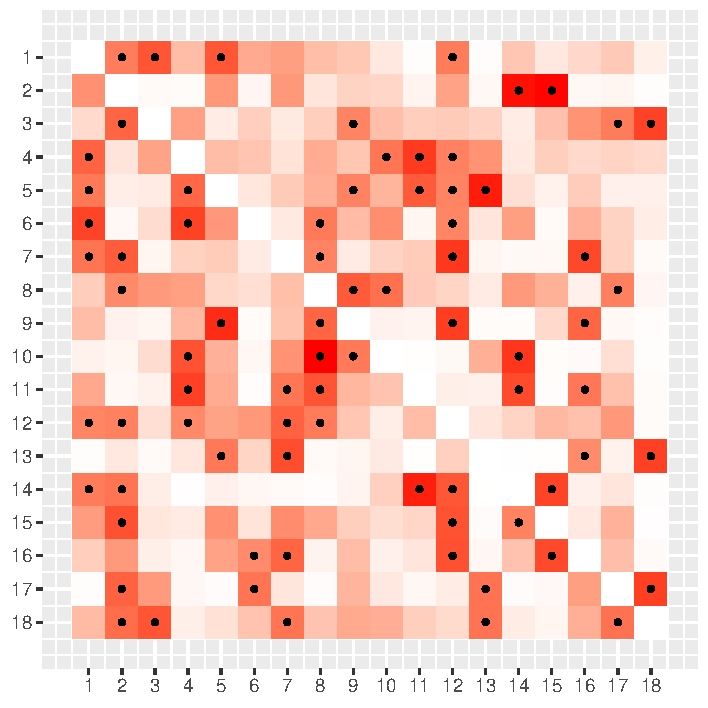
\includegraphics[width=\textwidth]{figures/S11-posterior-W.pdf}
		% \caption{S11 ($T$: 5, $F$: 0.4333)}
		\caption{S11 ($T$: 5)}
	\end{subfigure}
	\caption{Posterior Adjacency Matrices. (Varying $T$)}
	\label{fig:S-posterior-1}
\end{figure}
